\documentclass{article}
\usepackage[paperwidth=84.1cm,paperheight=118.9cm,margin=0cm]{geometry}
\usepackage{fontspec}
\usepackage{unicode-math}
\usepackage[brazilian]{babel}
\usepackage{ragged2e}
\usepackage{graphicx}
\usepackage{tikz}
\usetikzlibrary{arrows.meta}
\usepackage{qrcode}
\usepackage[hidelinks]{hyperref}
\setmainfont{Arial}
\setsansfont{Arial}
\setmathfont{latinmodern-math.otf}
\hypersetup{pdftitle={Algoritmos Exatos Para o Problema de Visita de Polígonos},pdfauthor={Gabriel Freire Ushijima; Ernesto G. Birgin},pdfsubject={34º SIICUSP, IME-USP}}
\pagestyle{empty}
\setlength{\parindent}{0pt}
\setlength{\parskip}{0.24em}
\definecolor{Ink}{HTML}{142D38}
\definecolor{Muted}{HTML}{47616A}
\definecolor{Accent}{HTML}{CF5A20}
\definecolor{Pale}{HTML}{EEF4F1}
\definecolor{Rule}{HTML}{C5D3CF}
\definecolor{MapDark}{HTML}{102C38}
\definecolor{Route}{HTML}{FFAD66}
\definecolor{FirstVisit}{HTML}{81D864}
\definecolor{LastVisit}{HTML}{1F7A73}
\newsavebox{\posterbox}
% Named, measured blocks make overflow checks reproducible after each edit.
\newcommand{\block}[5]{%
  \node[anchor=north west,inner sep=0] at (#2,#3) {%
  \sbox{\posterbox}{\begin{minipage}[t]{#4cm}\RaggedRight #5\end{minipage}}%
  \typeout{POSTERBLOCK #1 x=#2 y=#3 w=#4 h=\the\dimexpr\ht\posterbox+\dp\posterbox\relax}%
  \usebox{\posterbox}};}
\newcommand{\head}[2]{{\sffamily\bfseries\fontsize{42}{48}\selectfont\color{Accent}#1.\hspace{0.45cm}\color{Ink}#2\par}}
\newcommand{\bodytext}{\sffamily\mdseries\fontsize{26}{31}\selectfont\color{Ink}}
\newcommand{\bodymuted}{\sffamily\mdseries\fontsize{26}{31}\selectfont\color{Muted}}
\newcommand{\smalltext}{\bodymuted}
\newcommand{\tagtext}{\sffamily\bfseries\fontsize{25}{30}\selectfont\color{Accent}}
\newcommand{\metric}{\sffamily\bfseries\fontsize{66}{72}\selectfont\color{Accent}}
\begin{document}
\begin{tikzpicture}[remember picture,overlay,shift={(current page.north west)},x=1cm,y=-1cm]
  \fill[white] (0,0) rectangle (84.1,118.9);
  \fill[Ink] (0,0) rectangle (84.1,0.55);
  % Crop the SIICUSP image's white margins so the visible marks align by height.
  % The IME and SIICUSP marks are both 6.643 cm tall; FAPESP spans their row.
  \block{ime-logo}{67.686}{3.938}{5.015}{\centering
\includegraphics[height=6.643cm]{figures/ime-usp-vertical-logo.png}}
  \block{event-logo}{73.201}{3.938}{7.899}{
\includegraphics[trim={33bp 56bp 33bp 79bp},clip,width=\linewidth]{figures/siicusp34-logo-pt.png}}
  \block{funding-logo}{67.686}{11.6}{13.414}{
\includegraphics[width=\linewidth]{figures/fapesp-logo.png}}
  \block{funding}{67.686}{15.144}{13.414}{\raggedleft\sffamily\fontsize{26}{31}\selectfont\color{Muted}Processo 2025/13861-1\par}
  \block{title}{3}{4.4}{49.2}{\sffamily\bfseries\fontsize{88}{96}\selectfont\color{Ink}Algoritmos Exatos Para o\\Problema de Visita de Polígonos}
  \block{subtitle}{3}{11.3}{49.2}{\sffamily\fontsize{34}{41}\selectfont\color{Muted}Determinando caminhos mínimos para visitar regiões difíceis}
  \block{author}{3}{13.68}{37}{\sffamily\bfseries\fontsize{48}{55}\selectfont\color{Ink}Gabriel Freire Ushijima\par\vspace{0.08cm}\mdseries\fontsize{23}{27}\selectfont\color{Muted}\href{mailto:gabriel_ushijima@usp.br}{gabriel\_ushijima@usp.br}}
  \block{advisor}{30}{13.68}{51.1}{\sffamily\bfseries\fontsize{48}{55}\selectfont\color{Ink}Ernesto G. Birgin \mdseries(Orientador)\par\vspace{0.08cm}\fontsize{23}{27}\selectfont\color{Muted}\href{mailto:egbirgin@ime.usp.br}{egbirgin@ime.usp.br}}
  \draw[Rule,line width=1.1pt] (3,17.0) -- (81.1,17.0);
  \draw[Rule,line width=0.8pt] (41.95,18.3) -- (41.95,40.5);
  \draw[Rule,line width=0.8pt] (3,40.5) -- (81.1,40.5);
  \draw[Rule,line width=0.8pt] (33.25,41.4) -- (33.25,86.55);
  % Section 1 uses one half-page column; two fixed-order problems lead to free order.
  \block{intro-head}{3}{18.3}{38.2}{\head{1}{Introdução}}
  \block{intro-context}{3}{20.67}{38.2}{\bodytext Suponha que um drone parte da entrada do IME para fotografar institutos e outras regiões da USP. Precisamos escolher \textbf{a ordem das visitas e o ponto de contato} em cada região para minimizar o comprimento do caminho. Esse problema é exatamente o TPP de ordem livre, o foco desse projeto de pesquisa.}
  \fill[Pale,rounded corners=0.22cm] (3,25.7) rectangle (20.4,30.1);
  \draw[Rule,line width=1.0pt,rounded corners=0.22cm] (3,25.7) rectangle (20.4,30.1);
  \block{tsp}{3.55}{26.2}{16.3}{{\sffamily\bfseries\fontsize{27}{32}\selectfont\color{Accent}TSP}\par\vspace{0.10cm}\bodytext Menor ciclo que visita\\um conjunto de pontos.}
  \fill[Pale,rounded corners=0.22cm] (3,30.6) rectangle (20.4,36.18);
  \draw[Rule,line width=1.0pt,rounded corners=0.22cm] (3,30.6) rectangle (20.4,36.18);
  \block{tpp}{3.55}{31.1}{16.3}{{\sffamily\bfseries\fontsize{27}{32}\selectfont\color{Accent}TPP}\par\vspace{0.10cm}\bodytext Menor caminho que parte de $s$,\\visita uma sequência de polígonos\\em ordem e chega em $t$.}
  \fill[Accent!7,rounded corners=0.24cm] (22.8,26.9) rectangle (41.1,34.98);
  \draw[Accent!65,line width=1.2pt,rounded corners=0.24cm] (22.8,26.9) rectangle (41.1,34.98);
  \block{free-order}{23.45}{27.4}{17.0}{{\tagtext TPP de ordem livre}\par\vspace{0.14cm}\bodytext Menor caminho que parte de um ponto $s$,\\visita um conjunto de polígonos\\e chega em um ponto $t$.\par\vspace{0.10cm}\bodytext\bfseries Esse é o problema que resolvemos.}
  \draw[Accent,line width=1.8pt,-{Stealth[length=3mm]}] (20.4,27.9) -- (22.7,28.4);
  \draw[Accent,line width=1.8pt,-{Stealth[length=3mm]}] (20.4,33.39) -- (22.7,33.0);
  \block{evolution}{3}{36.6}{38.2}{\smalltext\textbf{Complementando o resumo:} O resumo apresentava o caso não convexo com ordem fixa. Após a submissão, concluímos a extensão para ordem livre.}

  % Section 2 presents the polynomial subproblem and the independent research story.
  \block{definitions-head}{42.7}{18.3}{38.4}{\head{2}{Trabalhos anteriores}}
  \block{prior-work}{42.7}{20.38}{38.4}{\tagtext Um subproblema polinomial\par\vspace{0.06cm}\bodytext Os três problemas são NP-difíceis. No entanto, para o TPP com polígonos convexos e ordem fixa, Dror et al. (2003) descrevem um algoritmo em $O(nk^2 \log n)$, depois melhorado por Tan \& Jiang (2017) para $O(nk^2)$. Aqui, $k$ é o número de polígonos e $n$ a soma dos vértices.}
  \block{competition-story}{42.7}{26.1}{38.4}{\tagtext Uma ideia natural e um contratempo\par\vspace{0.06cm}\bodytext Enumerar todas as ordens e peças convexas, acelerando a busca com branch and bound, parecia um caminho para o TPP de ordem livre. Começamos a explorar essa ideia; no entanto, poucos meses depois, Fekete et al. (2026) [3] publicaram uma abordagem semelhante para o TPP de ordem livre, tornando-se os primeiros a apresentar um algoritmo concreto para o problema.\par\vspace{0.10cm}\tagtext A comparação\par\vspace{0.06cm}\bodytext Eles resolvem o subproblema convexo com SOCP e Gurobi, um solver genérico comercial. Nós propomos resolver o subproblema convexo com um solver geométrico exato e especializado, adaptado de Dror et al. e Tan \& Jiang. Queríamos ganhar do solver deles nas próprias instâncias do artigo: com outra coleção, a diferença poderia vir dos casos, não dos métodos.}
  % The map now has a concise, concrete caption beneath it.
  \block{map-head}{3}{41.4}{29.5}{\head{3}{A USP como instância}}
  \block{usp-map}{3}{49.3}{29.5}{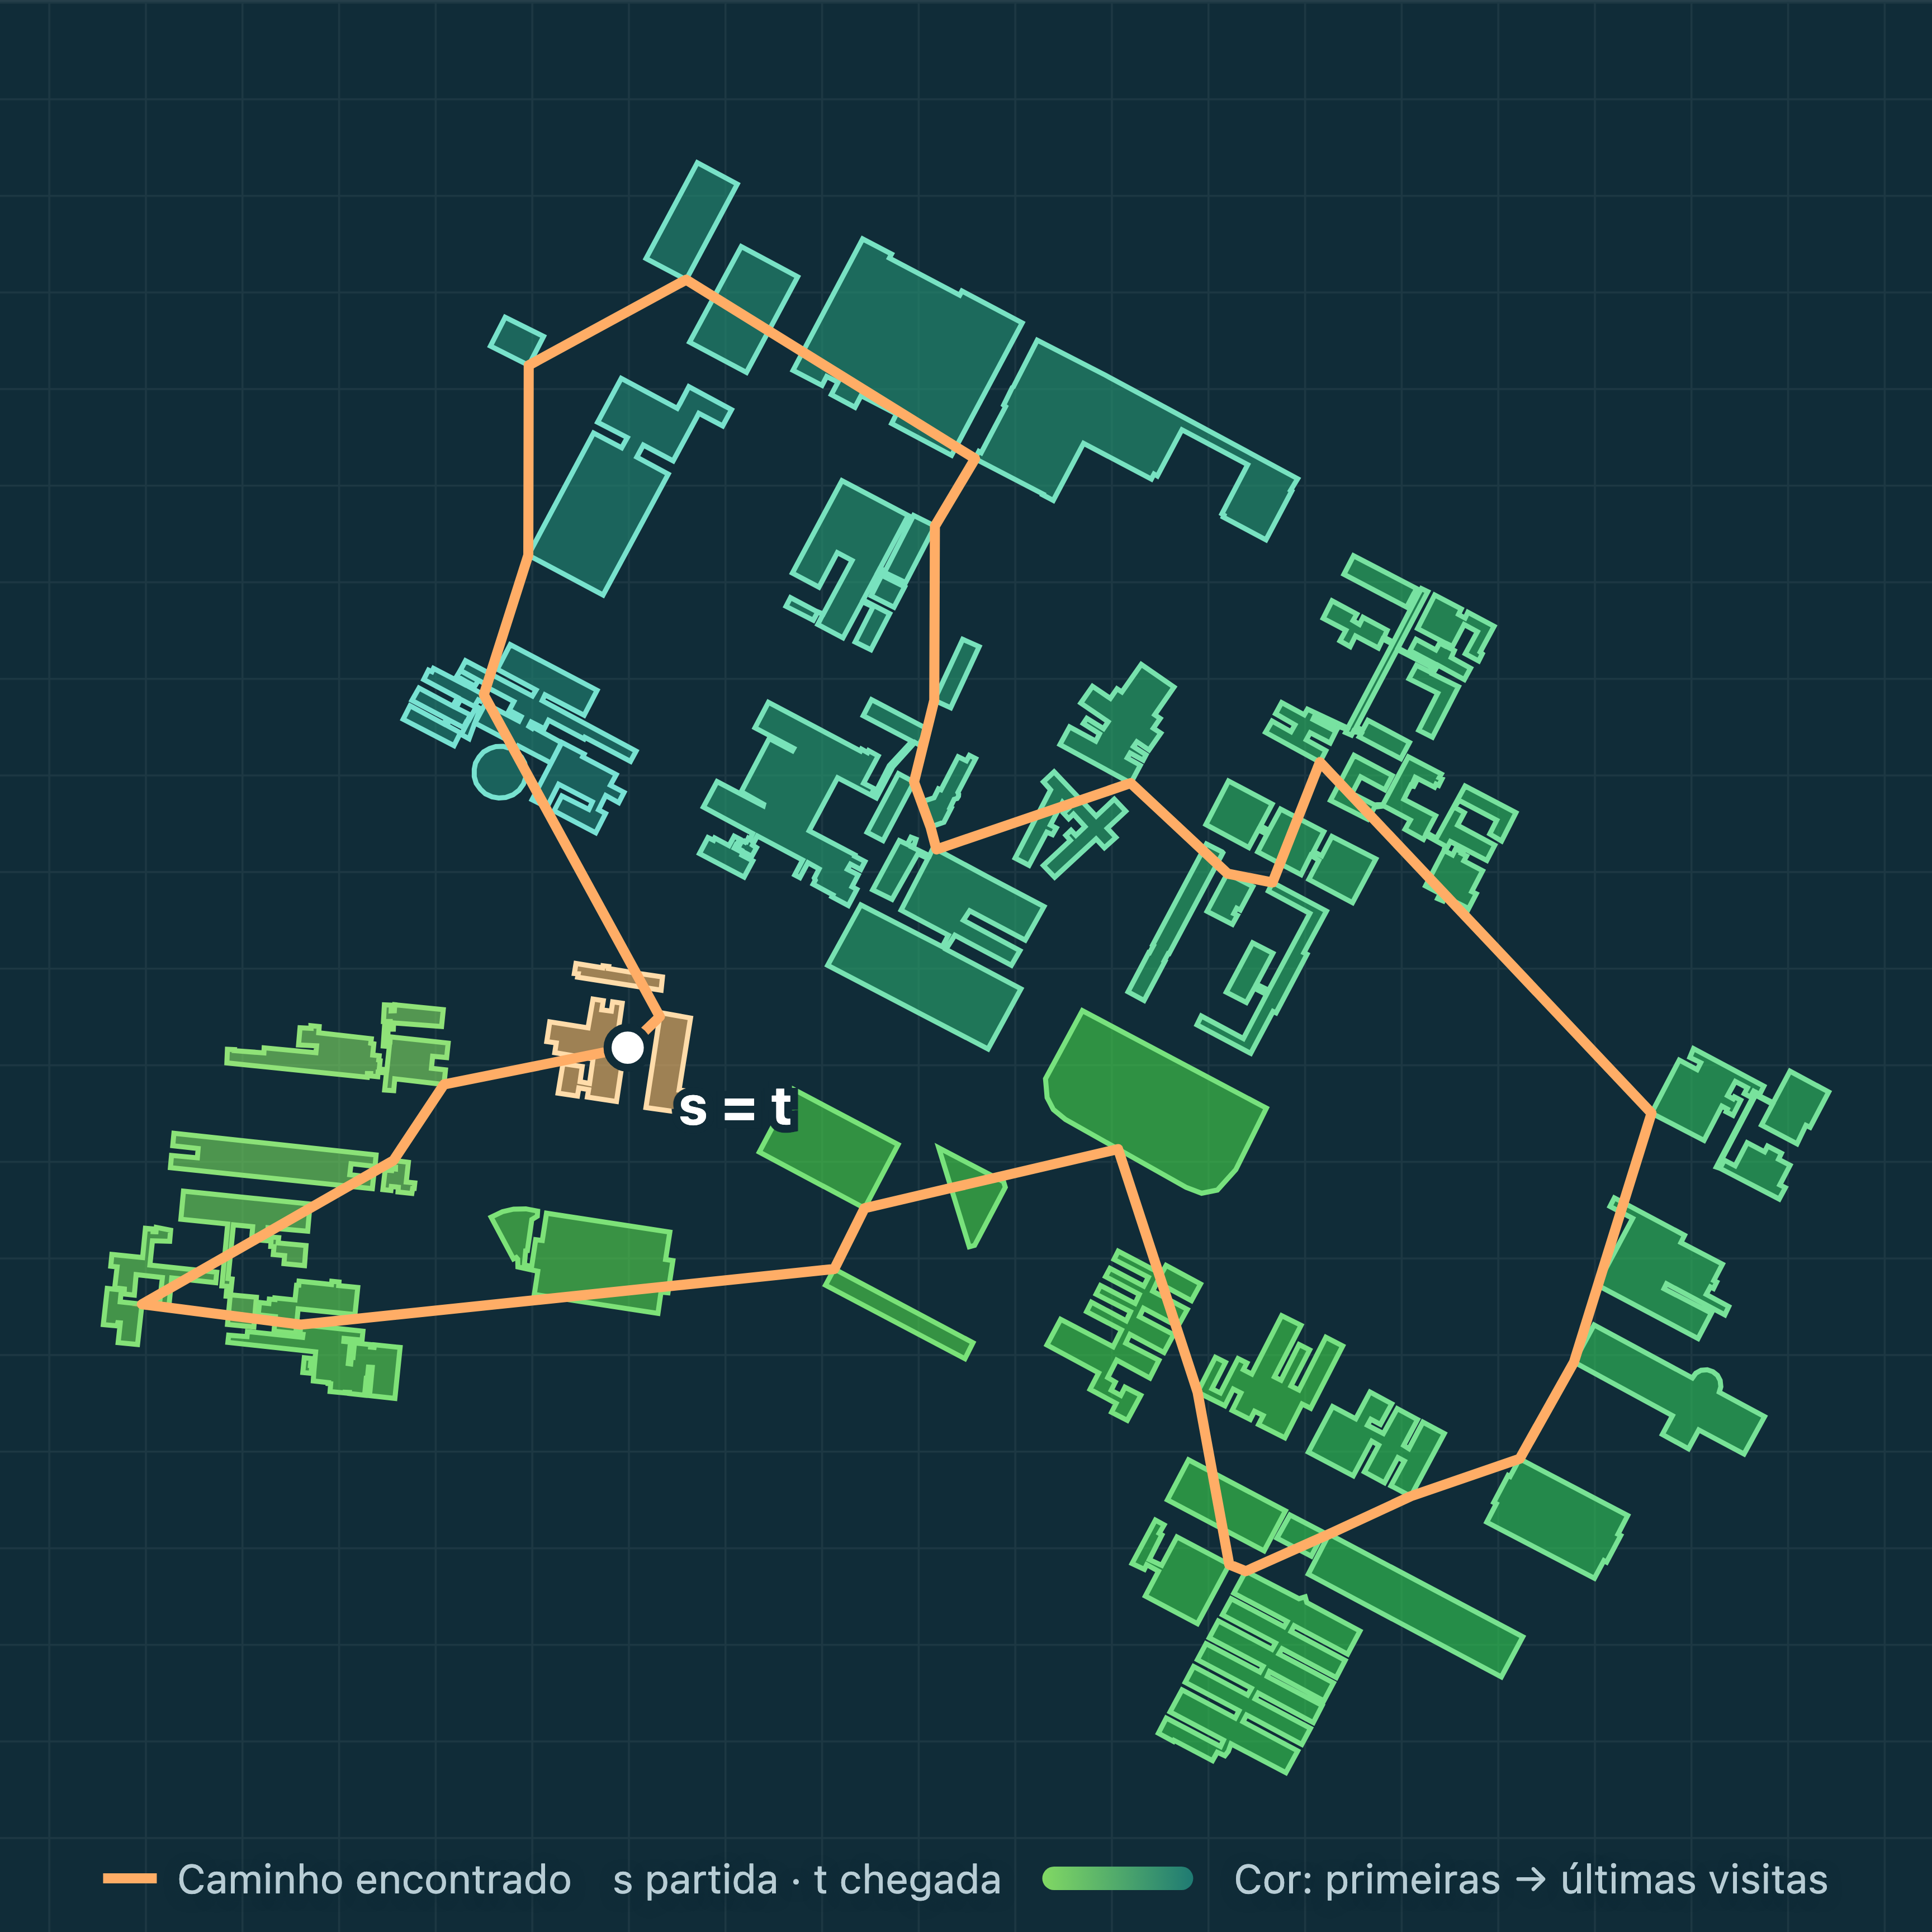
\includegraphics[width=\linewidth]{figures/usp-route-square.png}}
  \block{usp-context}{3}{43.3}{29.5}{\bodytext Esta instância usa 51 regiões da Cidade Universitária da USP, contornadas manualmente no QGIS sobre OpenStreetMap. O solver encontrou uma rota numericamente ótima, com 4,97 km, em 8,77 s. Regiões são alvos, não obstáculos; regras de voo não são modeladas.}

  \block{method-head}{34.0}{41.4}{47.1}{\head{4}{Buscar sem enumerar}}
  \block{search-principle}{34.0}{43.3}{47.1}{\bodytext\textbf{Como funciona a busca:} Cada nó relaxa os polígonos ainda não visitados: o fecho convexo dá limite inferior e a melhor rota viável, limite superior. Se esses limites não garantem a poda, inserimos uma região ou refinamos sua decomposição convexa.}
  % The six figures and captions below are taken from the published app.
  % Row 1: feasible route, partial order, and lower-bound pruning.
  \fill[white,rounded corners=0.22cm] (34.0,47) rectangle (49.5,65.7);
  \draw[Rule,line width=0.9pt,rounded corners=0.22cm] (34.0,47) rectangle (49.5,65.7);
  \fill[MapDark] (34.05,47.05) rectangle (49.45,54.15);
  \block{step1-art}{34.0}{47.15}{15.5}{\centering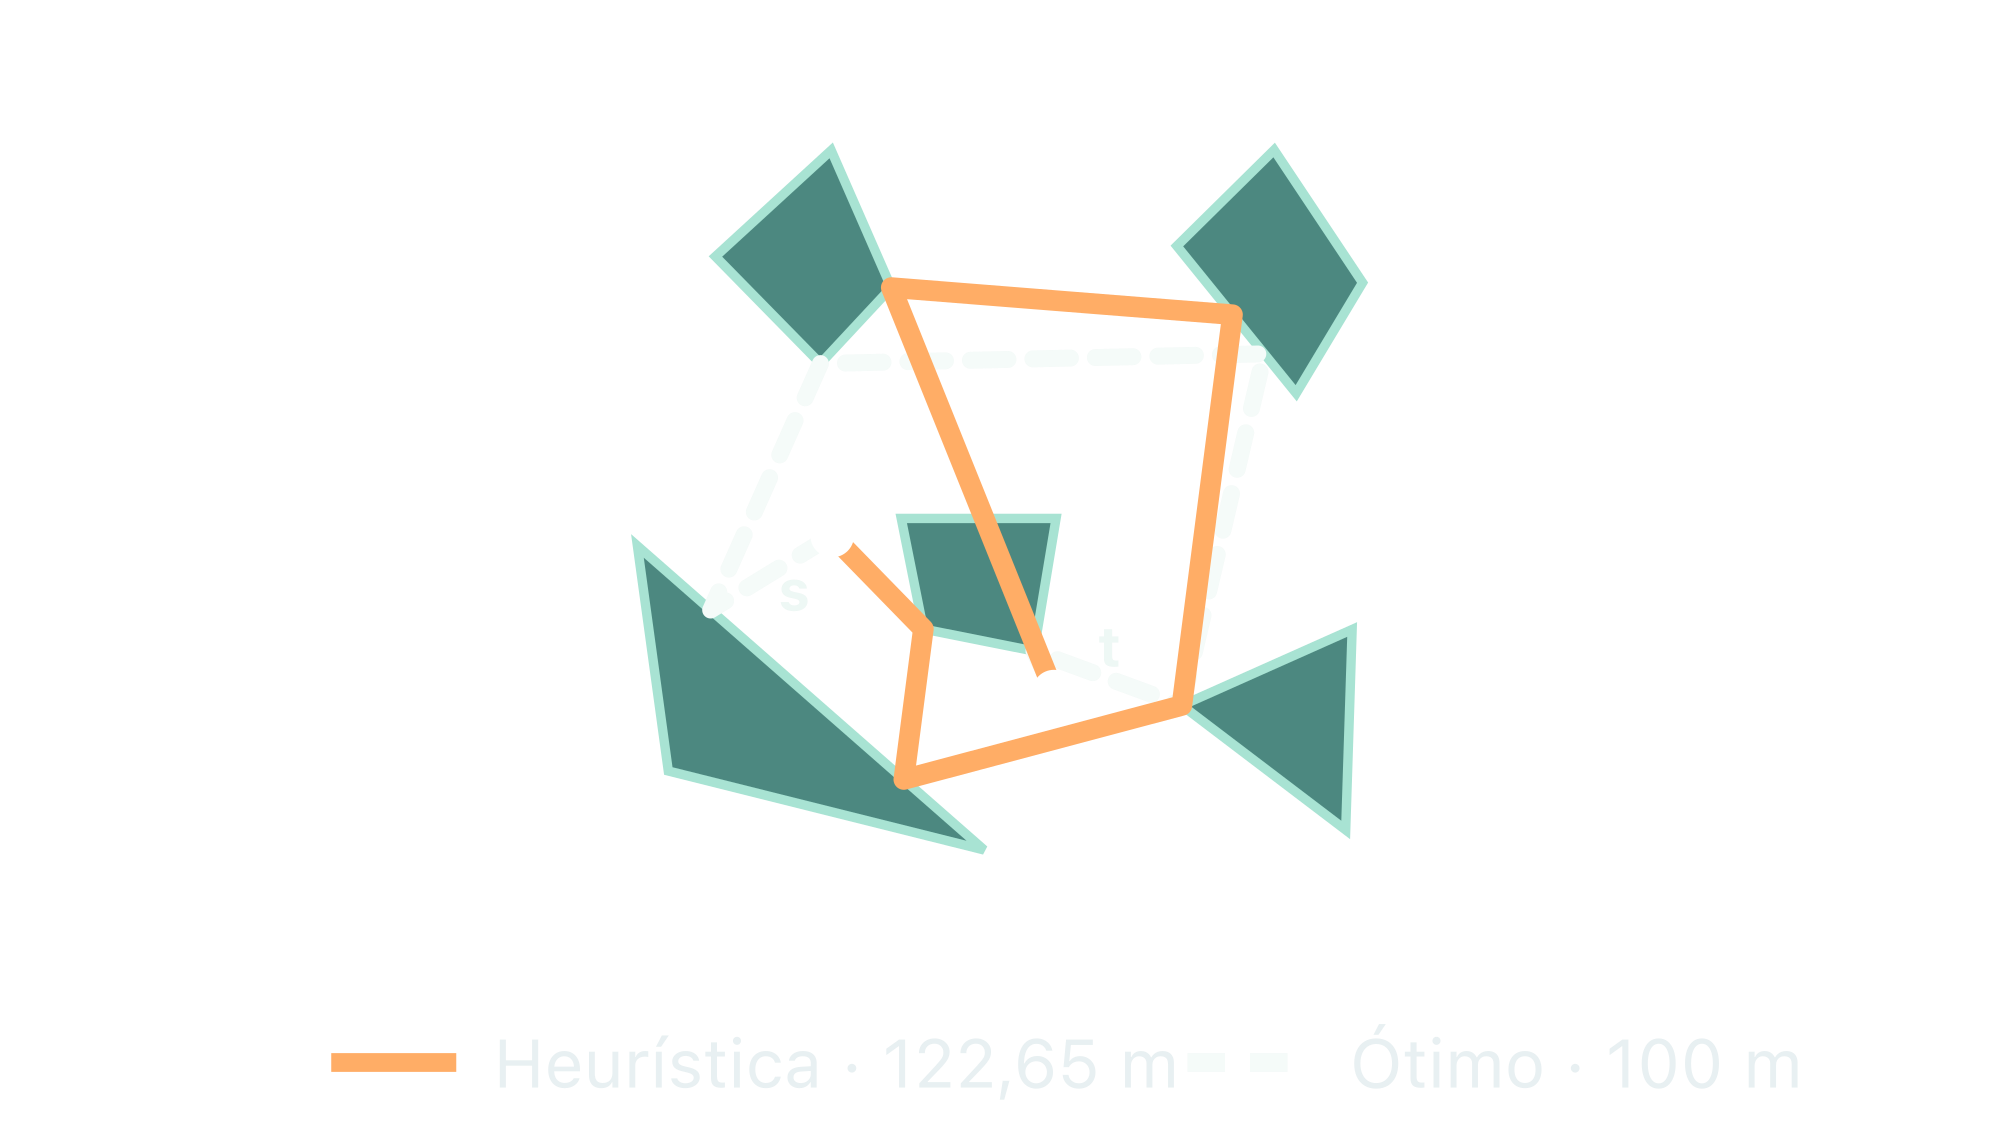
\includegraphics[height=6.9cm]{figures/method-step-01.png}}
  \block{step1-title}{34.55}{54.8}{14.4}{\bodytext\bfseries\color{Ink}01 · Encontrar uma rota viável}
  \block{step1-text}{34.55}{55.95}{14.4}{\bodytext\color{Muted}A heurística gulosa encontra uma rota viável e inicia o incumbente \textbf{$U$}. No desafio 1, ela não encontra o ótimo: a rota tracejada é mais curta e só aparece depois da busca.}

  \fill[white,rounded corners=0.22cm] (49.8,47) rectangle (65.3,65.7);
  \draw[Rule,line width=0.9pt,rounded corners=0.22cm] (49.8,47) rectangle (65.3,65.7);
  \fill[MapDark] (49.85,47.05) rectangle (65.25,54.15);
  \block{step2-art}{49.8}{47.15}{15.5}{\centering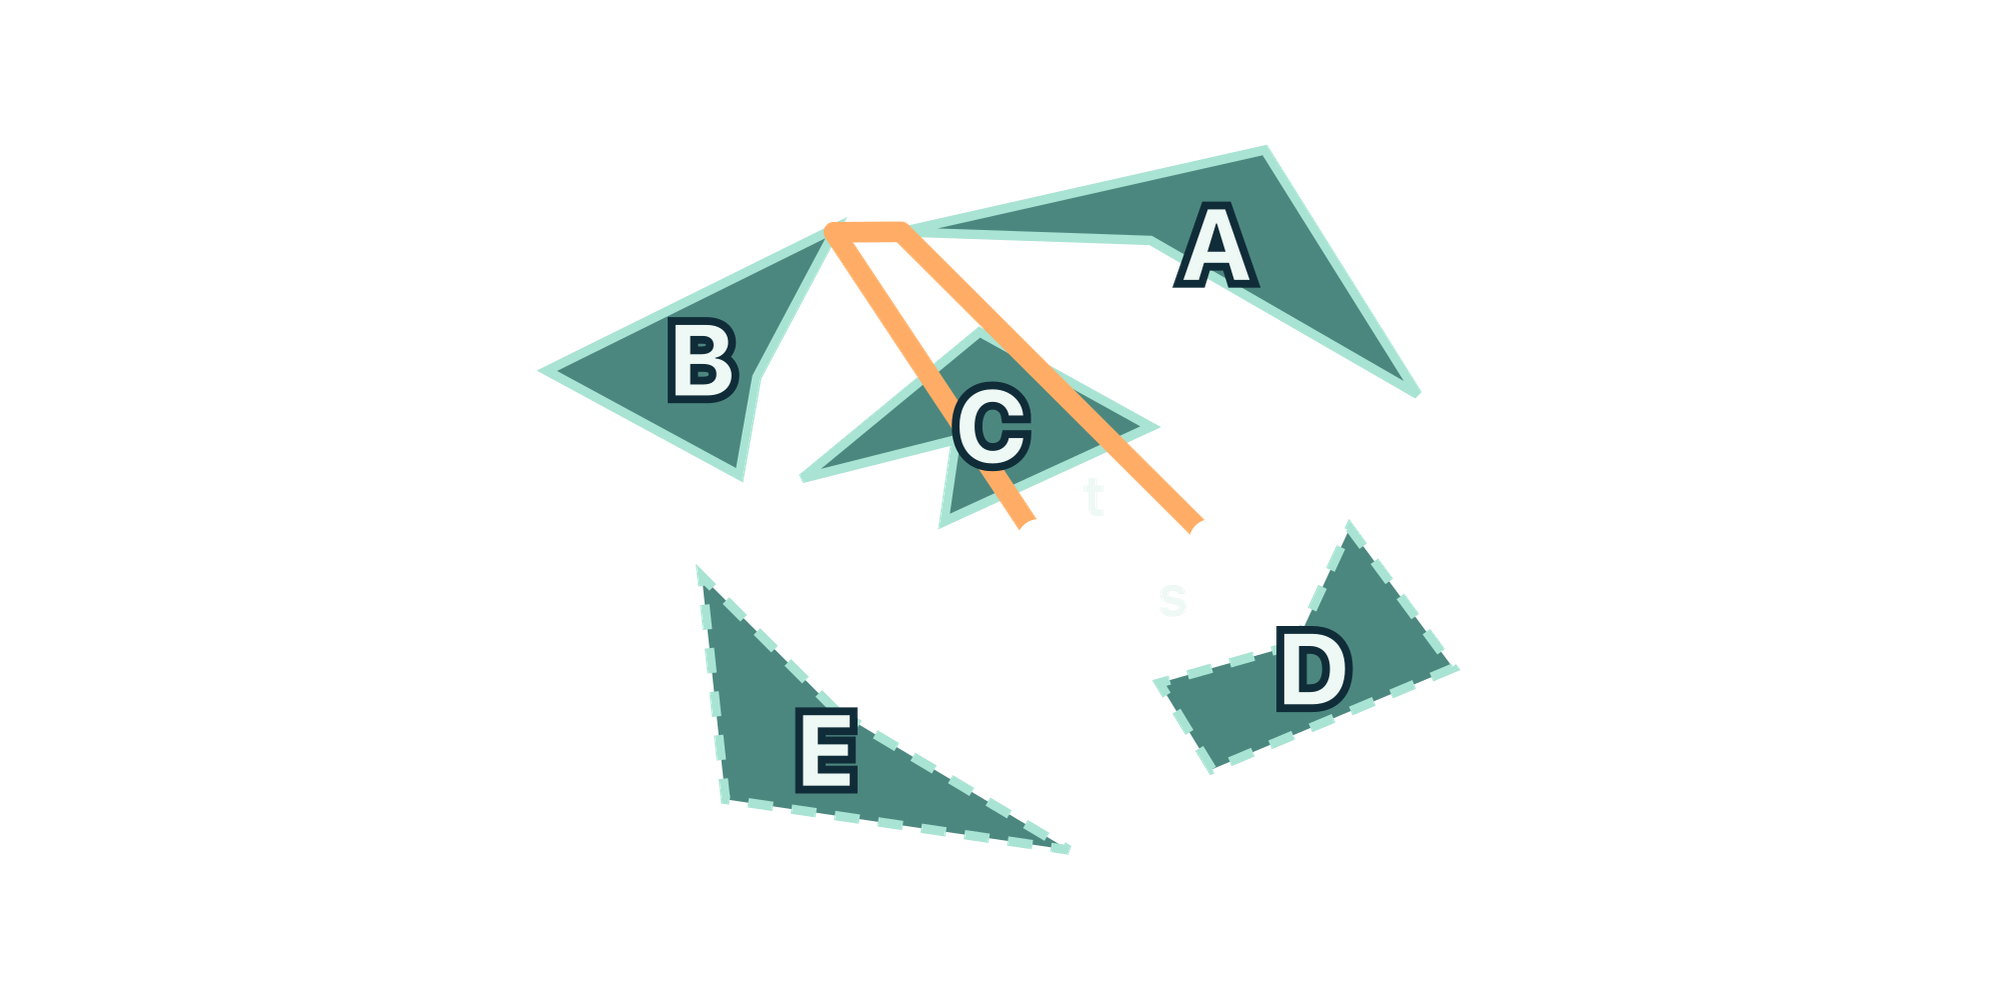
\includegraphics[height=6.9cm]{figures/method-step-02.png}}
  \block{step2-title}{50.35}{54.8}{14.4}{\bodytext\bfseries\color{Ink}02 · Manter ordenações parciais}
  \block{step2-text}{50.35}{55.95}{14.4}{\bodytext\color{Muted}Com apenas \textbf{A} e \textbf{B} fixados nessa ordem, a rota mínima também toca \textbf{C} por acaso, mas não toca \textbf{D} nem \textbf{E}. Só A e B fazem parte da sequência deste nó.}

  \fill[white,rounded corners=0.22cm] (65.6,47) rectangle (81.1,65.7);
  \draw[Rule,line width=0.9pt,rounded corners=0.22cm] (65.6,47) rectangle (81.1,65.7);
  \fill[MapDark] (65.65,47.05) rectangle (81.05,54.15);
  \block{step3-art}{65.6}{47.15}{15.5}{\centering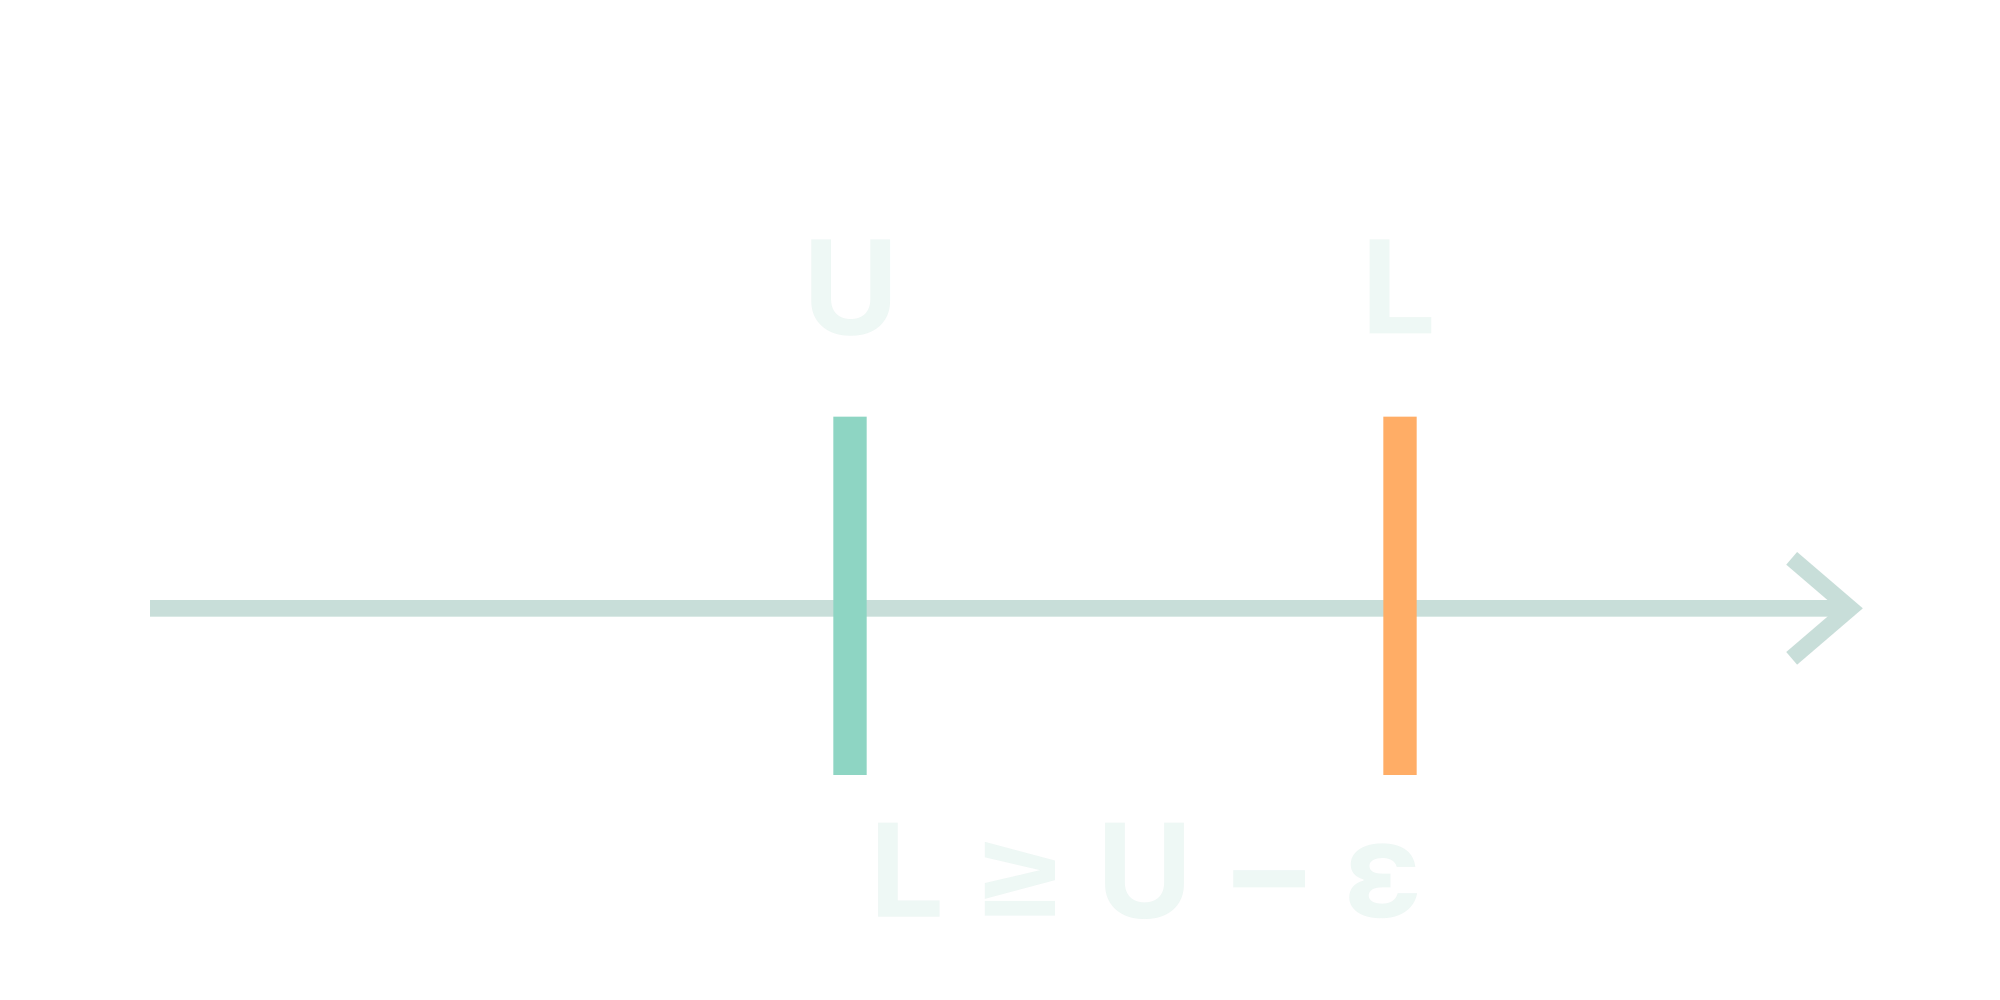
\includegraphics[height=6.9cm]{figures/method-step-03.png}}
  \block{step3-title}{66.15}{54.8}{14.4}{\bodytext\bfseries\color{Ink}03 · Podar pelo limite inferior}
  \block{step3-text}{66.15}{55.95}{14.4}{\bodytext\color{Muted}Dror et al. descrevem um algoritmo polinomial para alvos convexos disjuntos em ordem fixa. Nosso oráculo fornece um limite inferior certificado \textbf{$L$}; se ele alcança \textbf{$U$}, considerada a tolerância, o ramo não pode melhorar o incumbente.}

  % Row 2: incumbent update, insertion branching, and convex refinement.
  \fill[white,rounded corners=0.22cm] (34.0,66.15) rectangle (49.5,83.8);
  \draw[Rule,line width=0.9pt,rounded corners=0.22cm] (34.0,66.15) rectangle (49.5,83.8);
  \fill[MapDark] (34.05,66.2) rectangle (49.45,73.25);
  \block{step4-art}{34.0}{66.25}{15.5}{\centering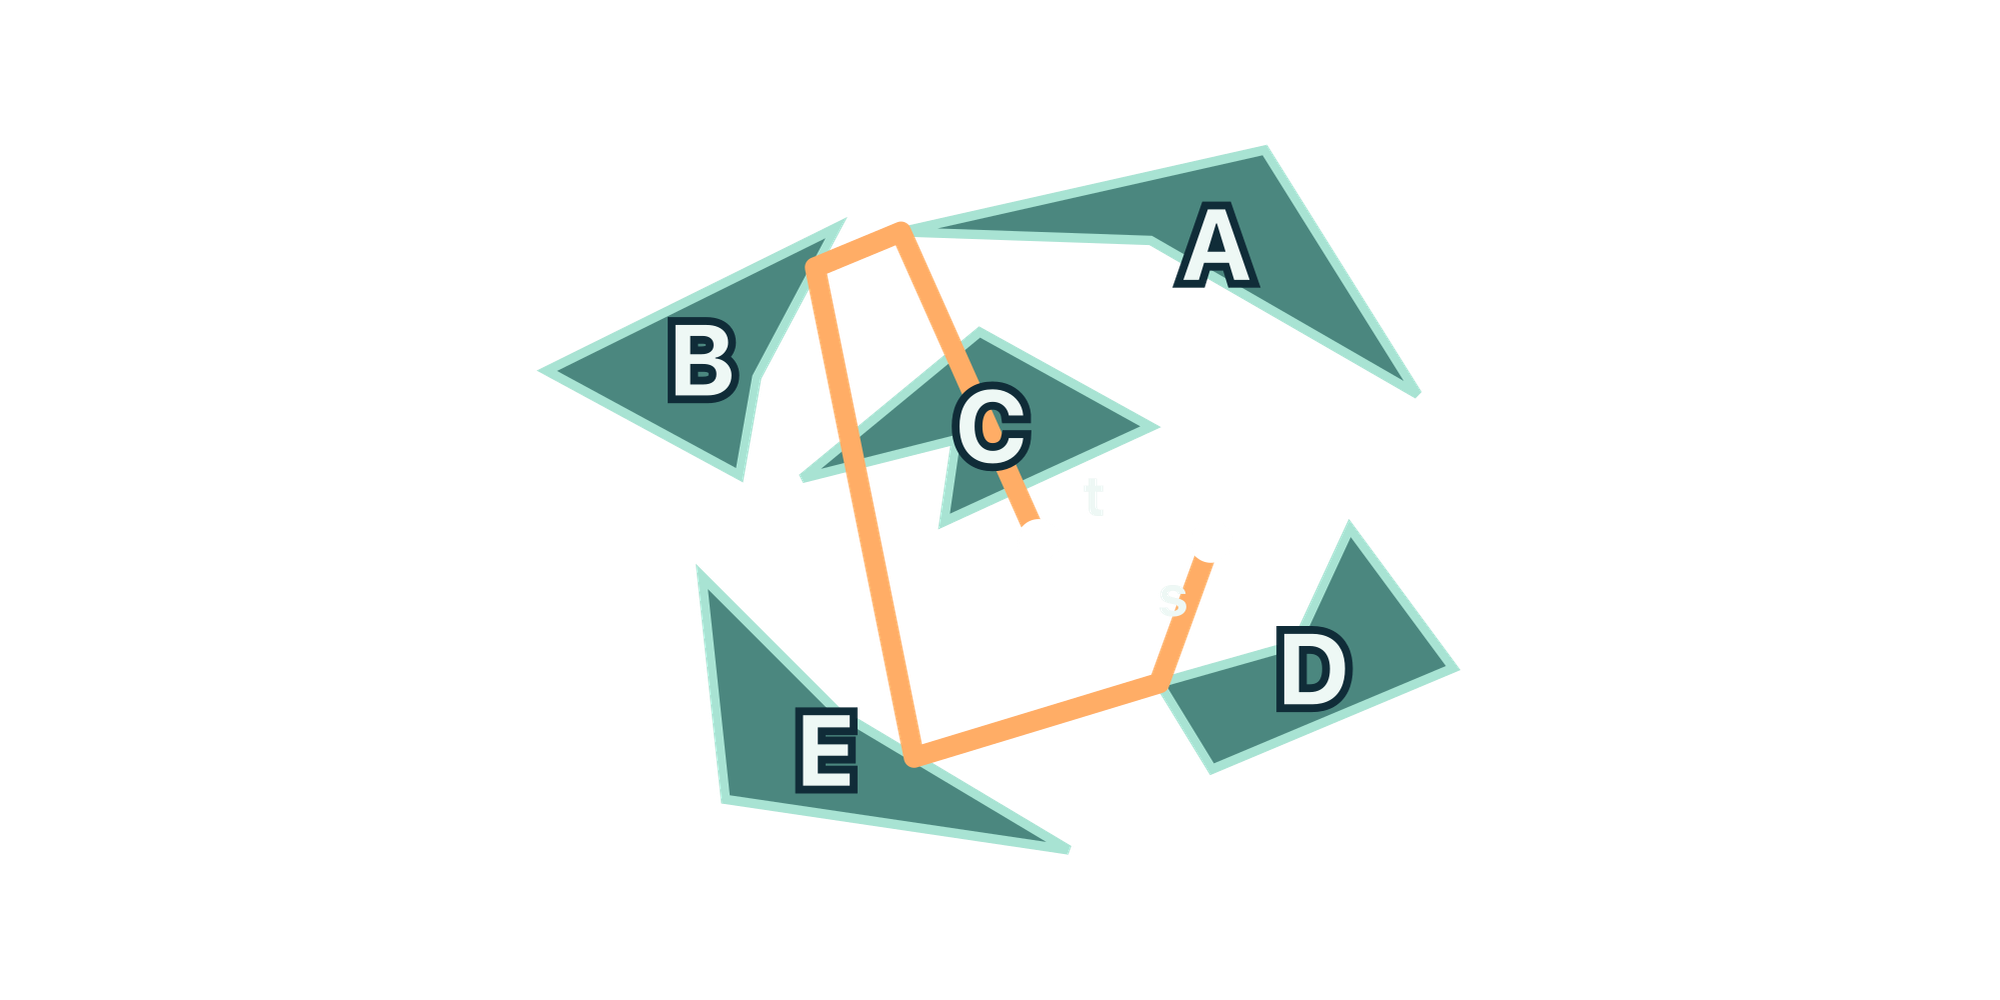
\includegraphics[height=6.9cm]{figures/method-step-04.png}}
  \block{step4-title}{34.55}{73.95}{14.4}{\bodytext\bfseries\color{Ink}04 · Atualizar o incumbente}
  \block{step4-text}{34.55}{74.95}{14.4}{\bodytext\color{Muted}Com todos os polígonos da instância incluídos, a rota final visita os cinco. Quando uma rota viável é mais curta que o incumbente atual, atualizamos \textbf{$U$}.}

  \fill[white,rounded corners=0.22cm] (49.8,66.15) rectangle (65.3,83.8);
  \draw[Rule,line width=0.9pt,rounded corners=0.22cm] (49.8,66.15) rectangle (65.3,83.8);
  \fill[MapDark] (49.85,66.2) rectangle (65.25,73.25);
  \block{step5-art}{49.8}{66.25}{15.5}{\centering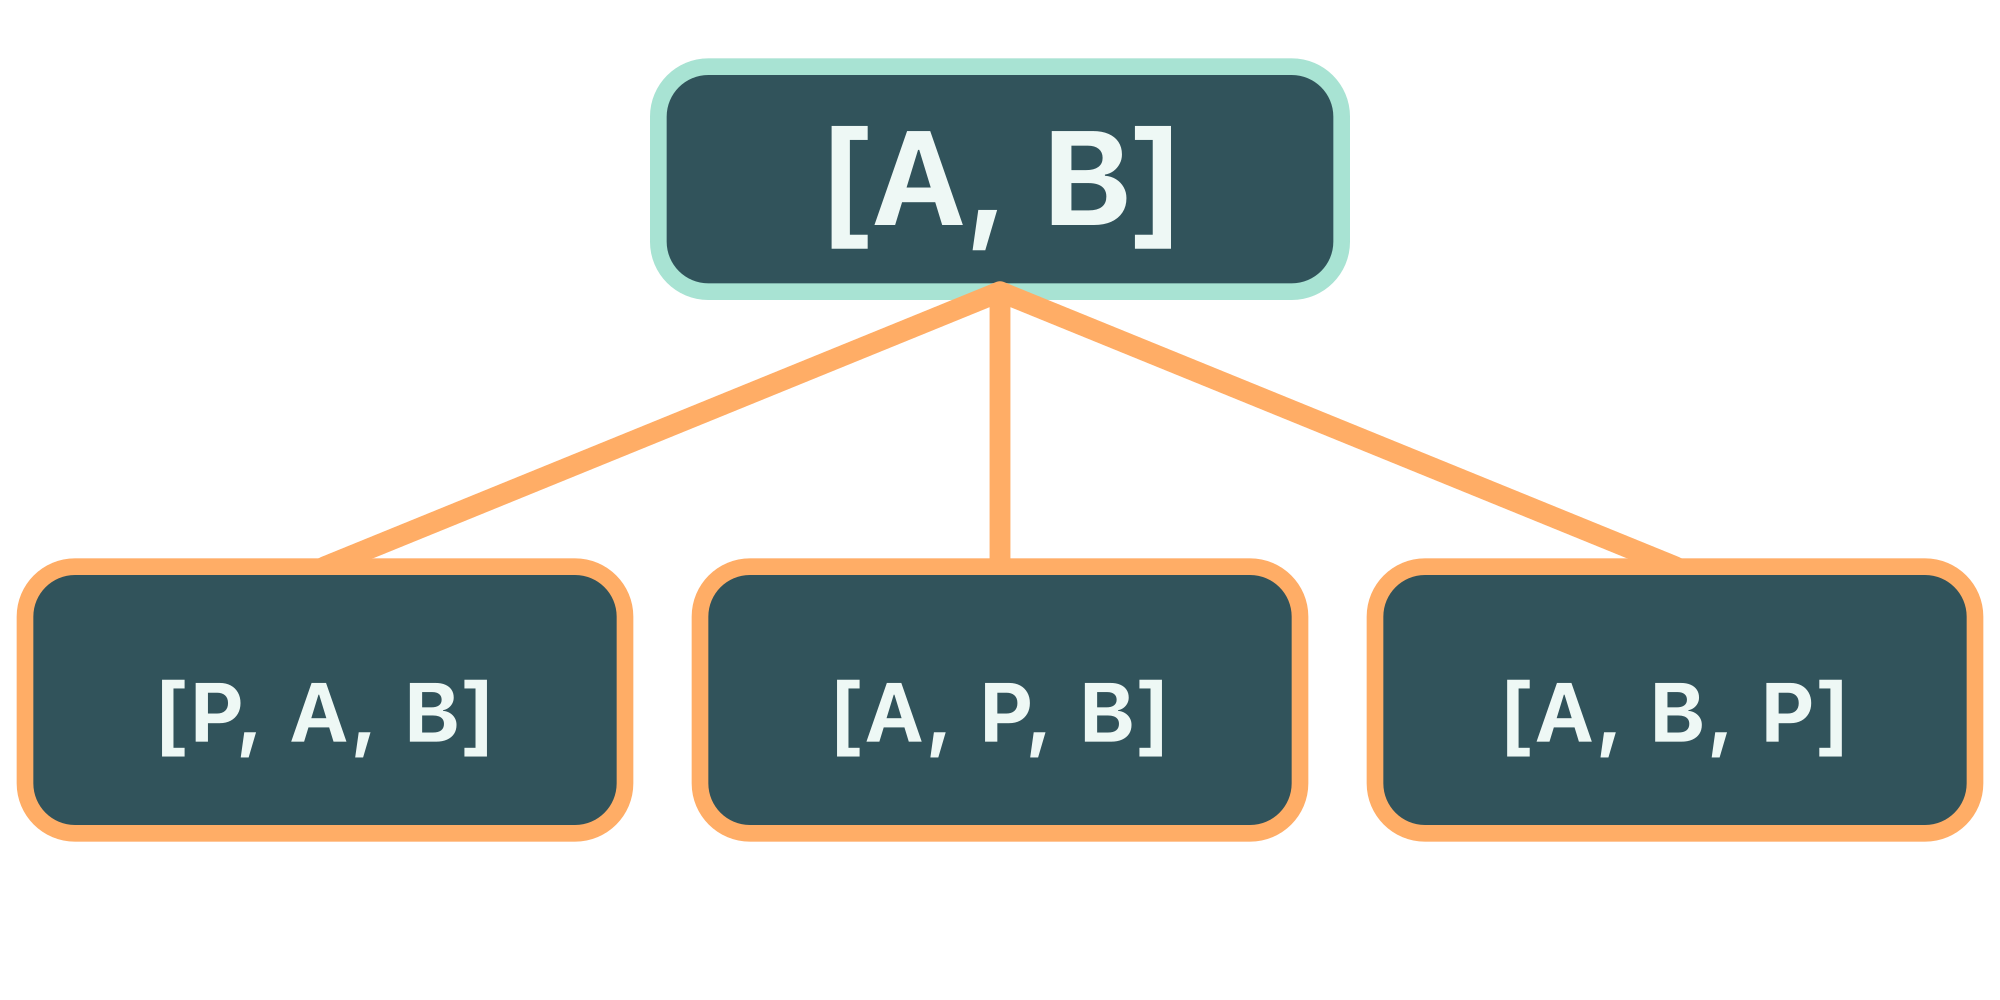
\includegraphics[height=6.9cm]{figures/method-step-05.png}}
  \block{step5-title}{50.35}{73.95}{14.4}{\bodytext\bfseries\color{Ink}05 · Gerar as $\mathbf{m + 1}$ inserções}
  \block{step5-text}{50.35}{74.95}{14.4}{\bodytext\color{Muted}Escolhemos o polígono não visitado mais distante. Com $m$ polígonos na sequência, inserir $P$ gera $m+1$ posições: antes, entre ou depois dos já ordenados.}

  \fill[white,rounded corners=0.22cm] (65.6,66.15) rectangle (81.1,83.8);
  \draw[Rule,line width=0.9pt,rounded corners=0.22cm] (65.6,66.15) rectangle (81.1,83.8);
  \fill[MapDark] (65.65,66.2) rectangle (81.05,73.25);
  \block{step6-art}{65.6}{66.25}{15.5}{\centering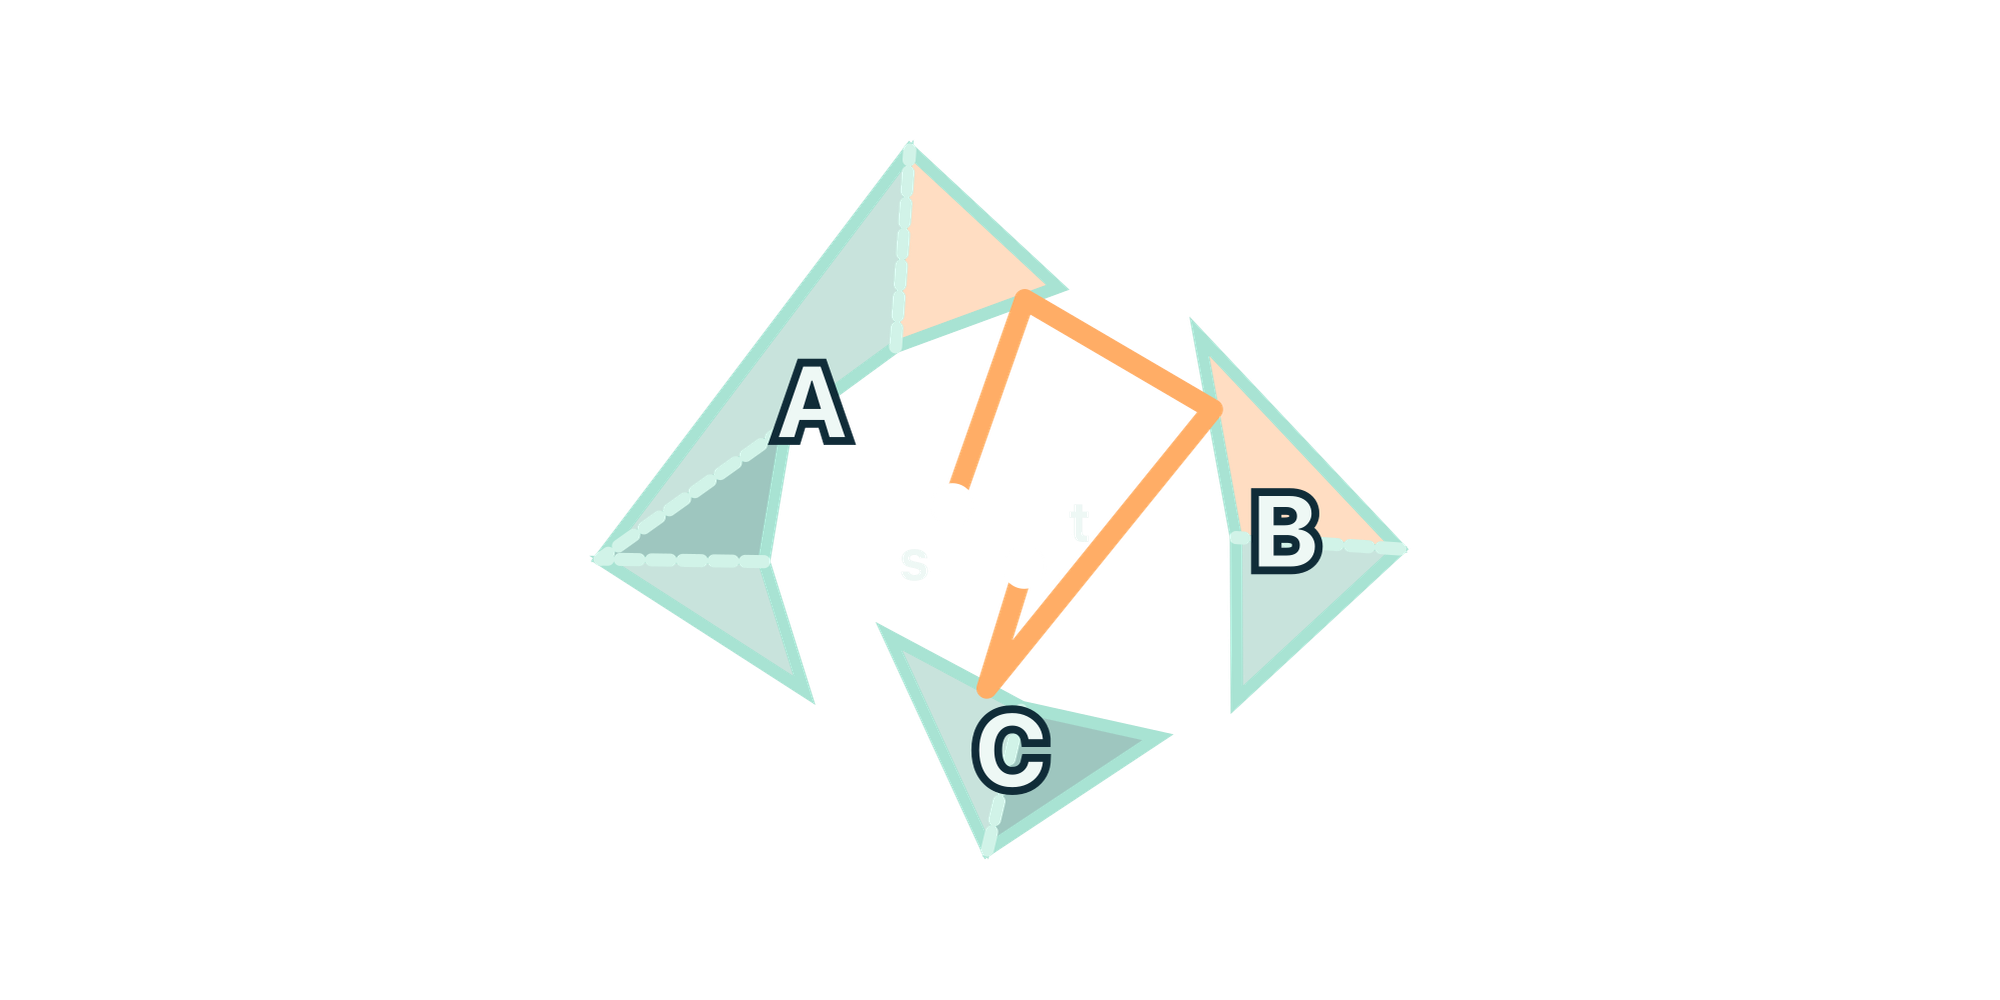
\includegraphics[height=6.9cm]{figures/method-step-06.png}}
  \block{step6-title}{66.15}{73.95}{14.4}{\bodytext\bfseries\color{Ink}06 · Refinar em peças convexas}
  \block{step6-text}{66.15}{74.95}{14.4}{\bodytext\color{Muted}No desafio 2, os três polígonos são decompostos em peças convexas. Para cada um, a busca ramifica entre as peças; o caminho mostrado toca uma peça de cada polígono.}
  \block{method-provenance}{34.0}{84.15}{47.1}{\smalltext Decomposição convexa: implementamos Greene [4]. Inserção e refinamento adaptados de Fekete et al. [3].}


  % Results and the app share the final content row.
  \draw[Rule,line width=1.1pt] (3,86.9) -- (81.1,86.9);
  \block{results-head}{3}{87.7}{46.0}{\head{5}{Resultados no corpus de Fekete et al. e conclusão}}
  \block{app-head}{52}{87.7}{29.1}{\head{6}{Tente você mesmo!}}
  \draw[Rule,line width=0.8pt] (50.5,87.7) -- (50.5,111.6);

  \block{comparison-context}{3}{89.95}{45.9}{\bodytext Comparamos nosso solver ao de Fekete et al. nas instâncias do artigo deles, com uma thread e limite de 6 h por caso. Tempo e speedup usam os 550 casos concluídos por ambos; a precisão usa as trajetórias disponíveis.}
  \fill[white,rounded corners=0.30cm] (3,93.55) rectangle (48.9,100.1);
  \draw[Rule,line width=1.0pt,rounded corners=0.30cm] (3,93.55) rectangle (48.9,100.1);
  \draw[Route,line width=4.0pt] (3.3,93.60) -- (17.95,93.60);
  \draw[LastVisit,line width=4.0pt] (18.65,93.60) -- (33.25,93.60);
  \draw[Ink,line width=4.0pt] (33.95,93.60) -- (48.6,93.60);
  \draw[Rule,line width=0.8pt] (18.3,94.0) -- (18.3,99.2);
  \draw[Rule,line width=0.8pt] (33.6,94.0) -- (33.6,99.2);
  \block{speedup}{3.7}{94.3}{13.8}{\metric 5,11×\par\vspace{0.12cm}\bodytext\textbf{Speedup mediano}\par\smalltext Fekete / nosso.}
  \block{faster}{18.9}{94.3}{13.9}{\metric 492 / 550\par\vspace{0.12cm}\bodytext\textbf{Casos mais rápidos}\par\smalltext Nosso solver; Fekete venceu nos outros 58.}
  \block{completion}{34.2}{94.3}{13.9}{\metric 558 / 558\par\vspace{0.12cm}\bodytext\textbf{Ótimos certificados}\par\smalltext Nosso solver. Fekete concluiu 550/558 com gap ≤ 0,1\%.}

  \fill[Accent!7,rounded corners=0.20cm] (3,100.45) rectangle (48.9,105.0);
  \draw[Accent!45,line width=0.8pt,rounded corners=0.20cm] (3,100.45) rectangle (48.9,105.0);
  \block{case49-title}{3.7}{100.7}{44.5}{\tagtext Caso 49 · 60 regiões}
  \draw[Rule,line width=0.8pt] (25.95,101.9) -- (25.95,104.7);
  \block{case49-search-space}{3.7}{101.9}{20.8}{\sffamily\bfseries\fontsize{48}{54}\selectfont\color{Accent}$1{,}56\times10^{117}$\par\vspace{0.02cm}\smalltext combinações formais}
  \block{case49-runtime}{26.6}{101.9}{21.6}{\sffamily\bfseries\fontsize{48}{54}\selectfont\color{Accent}2,47 s\par\vspace{0.02cm}\smalltext Uma thread; solver não enumerou.}

  \fill[Pale,rounded corners=0.20cm] (3,105.35) rectangle (48.9,111.6);
  \draw[Rule,line width=0.8pt,rounded corners=0.20cm] (3,105.35) rectangle (48.9,111.6);
  \block{conclusion-title}{3.7}{105.7}{44.5}{\tagtext Conclusão}
  \block{conclusion-text}{3.7}{106.8}{44.5}{\bodytext Nas instâncias de Fekete et al., nosso solver certificou o ótimo em 558/558 casos e foi mais rápido em 492 dos 550 concluídos por ambos.}
  \block{contact-summary}{3.7}{109.15}{44.5}{\smalltext P95 da distância mínima entre a rota e cada região visitada: 0 m (nosso, 16.303 visitas); 9,31 μm (Fekete, 15.883).}

  \draw[Rule,line width=0.8pt,rounded corners=0.20cm] (52,90.1) rectangle (81.1,111.6);
  \draw[Accent,line width=3.0pt] (52.2,90.1) -- (80.9,90.1);
  \block{app-intro}{52.7}{90.95}{19.2}{\bodytext Explore as rotas da USP, das 32 subprefeituras de São Paulo e das 27 unidades federativas do Brasil. No web app, a explicação do algoritmo é muito mais aprofundada!}
  \block{qr}{72.4}{90.8}{8.4}{\qrcode[level=H,height=8.4cm]{https://yushipy.github.io/TouringPolygons/apps/siicusp34/}}
  \block{app-link}{52.7}{96.6}{19.2}{\sffamily\bfseries\fontsize{18}{22}\selectfont\color{Accent}\href{https://yushipy.github.io/TouringPolygons/apps/siicusp34/}{yushipy.github.io/TouringPolygons/apps/siicusp34/}}
  \draw[Rule,line width=0.8pt] (66.55,99.6) -- (66.55,107.4);
  \draw[Rule,line width=0.8pt] (52.7,104.3) -- (80.4,104.3);
  \block{app-usp-title}{52.7}{99.8}{13.3}{\tagtext USP, SP e Brasil}
  \block{app-usp-detail}{52.7}{100.8}{13.3}{\bodytext Instâncias separadas do corpus.}
  \block{app-challenges-title}{67.05}{99.8}{13.3}{\tagtext 3 desafios}
  \block{app-challenges-detail}{67.05}{100.8}{13.3}{\bodytext Monte você mesmo a rota e tente encontrar o ótimo!}
  \block{app-corpus-title}{52.7}{104.6}{13.3}{\tagtext 558 instâncias}
  \block{app-corpus-detail}{52.7}{105.6}{13.3}{\bodytext Explore \textbf{todos} os casos do artigo de Fekete et al.}
  \block{app-trace-title}{67.05}{104.6}{13.3}{\tagtext Simulação passo a passo}
  \block{app-trace-detail}{67.05}{105.6}{13.3}{\bodytext Veja uma simulação passo a passo do algoritmo, detalhando cada etapa do algoritmo.}
  % References and credits; the digital PDF keeps live links.
  \draw[Rule,line width=0.8pt] (3,112.1) -- (81.1,112.1);
  \block{references-col-1}{3}{112.6}{24.7}{\sffamily\fontsize{26}{31}\selectfont\color{Muted}\textbf{Referências}\par
  [1] Dror et al. \href{https://doi.org/10.1145/780542.780612}{\emph{Touring a Sequence of Polygons}}. STOC, 2003.\par
  [2] Tan; Jiang. \href{https://doi.org/10.1007/978-3-319-55911-7_44}{\emph{Efficient Algorithms for Touring a Sequence of Convex Polygons and Related Problems}}. TAMC, 2017.}
  \block{references-col-2}{29.7}{112.6}{24.7}{\sffamily\fontsize{26}{31}\selectfont\color{Muted}
  [3] Fekete et al. \href{https://doi.org/10.4230/LIPIcs.SoCG.2026.46}{\emph{A Branch-and-Bound Algorithm for the Traveling Salesman Problem with Difficult Neighborhoods}}. SoCG, 2026.}
  \block{references-col-3}{56.4}{112.6}{24.7}{\sffamily\fontsize{26}{31}\selectfont\color{Muted}
  [4] Greene. \emph{The Decomposition of Polygons into Convex Parts}. Computational Geometry, 1983.\par\vspace{0.12cm}
  O autor declara não haver conflito de interesses.}
\end{tikzpicture}
\end{document}
